\mainsection{\the\numexpr \thechapter + 1 \relax}{Introduction aux variables}{dd/mm/yyyy}
%voir : http://www.monlyceenumerique.fr/snt_seconde/python/python_en_seconde.html
%voir : https://www.maths-cours.fr/cours/python-au-lycee-1/
%http://info-mounier.fr/snt/python/introduction_variables.php
\vspace{-0.8cm}
\section{Le concept de variable}
\begin{wrapfigure}[]{r}{0.3\textwidth}
	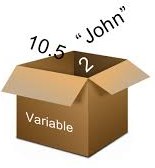
\includegraphics[trim=0 0 0 45,width=0.28\textwidth]{Images/variables/variables}
\end{wrapfigure}
Le but d'un programme est de transformer de l'information. En général, un programme va commencer par stocker en mémoire les données d’entrée qui seront utilisées lors des étapes de traitement. Pour accéder à ces espaces de stockage et savoir quelle genre d'information ils contiennent, il va falloir leur attribuer un nom (ou \textbf{identifiant}) ainsi qu'un \textbf{type}. Pour finir, ces données vont varier au fil de l'exécution du programme, c'est pourquoi on les appelle des \textbf{variables}. Chaque fois qu'on modifie la valeur d'une variable, on dit qu'on lui \textbf{affecte} une nouvelle valeur.
\begin{mydefinitions}
	\item  Une \textbf{variable} est un nom associé à un emplacement de la mémoire. C’est comme une boîte que l’on identifie par une étiquette. On dit aussi que le \textbf{nom de la variable est son identifiant}.
	\item Une \textbf{affectation} est l’attribution d’une valeur (d’un contenu) à une variable
\end{mydefinitions}
Pour résumer, une variable est décrite par
\begin{itemize}
	\item Un \textbf{identifiant} unique qui la désigne.
	\item Un \textbf{type} qui définit de quel « genre » est l’information associée.
	\item Une \textbf{valeur} qui doit respecter le type.
\end{itemize}


\vspace{1cm}
\act Indiquez le type des variables permettant de stocker (sur votre smartphone) les informations suivantes :
\begin{enumerate}[label=\alph*)]
	\item le nom d’un contact
	\item le numéro de téléphone d’un contact
	\item un SMS
	\item l’heure du réveil
	\item le code de votre de votre compte eduge.
	\item le pourcentage affiché de batterie restante
	\item la note de votre dernière évaluation de Mathématiques
\end{enumerate}

\vspace{1cm}

\newpage

\begin{wrapfigure}[]{r}{0.3\textwidth}
	\centering
	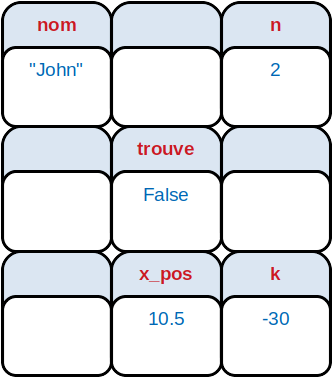
\includegraphics[width=0.28\textwidth]{Images/variables/memoire}
	\caption{\small Représentation d'une mémoire d'ordinateur  comme des boîtes. Lorsqu'une variable est crée la boite obtient une \textit{étiquette} (en rouge) et une valeur (en bleu).}
\end{wrapfigure}
Il faut imaginer la mémoire de l’ordinateur comme une grosse armoire avec plein de petites boîtes. 
Certaines de ces boîtes ont un nom (une étiquette) : ce sont des variables, et elles peuvent contenir une valeur. Chaque fois que l'on a besoin de stocker une donnée on va créer une nouvelle variable, en programmation on dira que l'on \textbf{déclare} une variable.

En \py la déclaration d’une variable (et son typage) se fait dynamiquement à l’exécution du programme dès que cette variable apparaît dans une ligne de code. En fait, il suffit d'une \textbf{affectation} en utilisant le symbole "\lstinline{=}". Le code
\begin{lstlisting}[numbers=none]
myInt = 4
myString = "hello"
myReal = 2.5
\end{lstlisting}
crée 3 variables avec comme identifiant \lstinline{myInt}, \lstinline{myString} et \lstinline{myFloat} qui sont de type \lstinline{int}, \lstinline{str} et \lstinline{float} et qui contiennent les données \lstinline{4}, \lstinline{"hello"} et \lstinline{2.5}. 
\begin{center}
	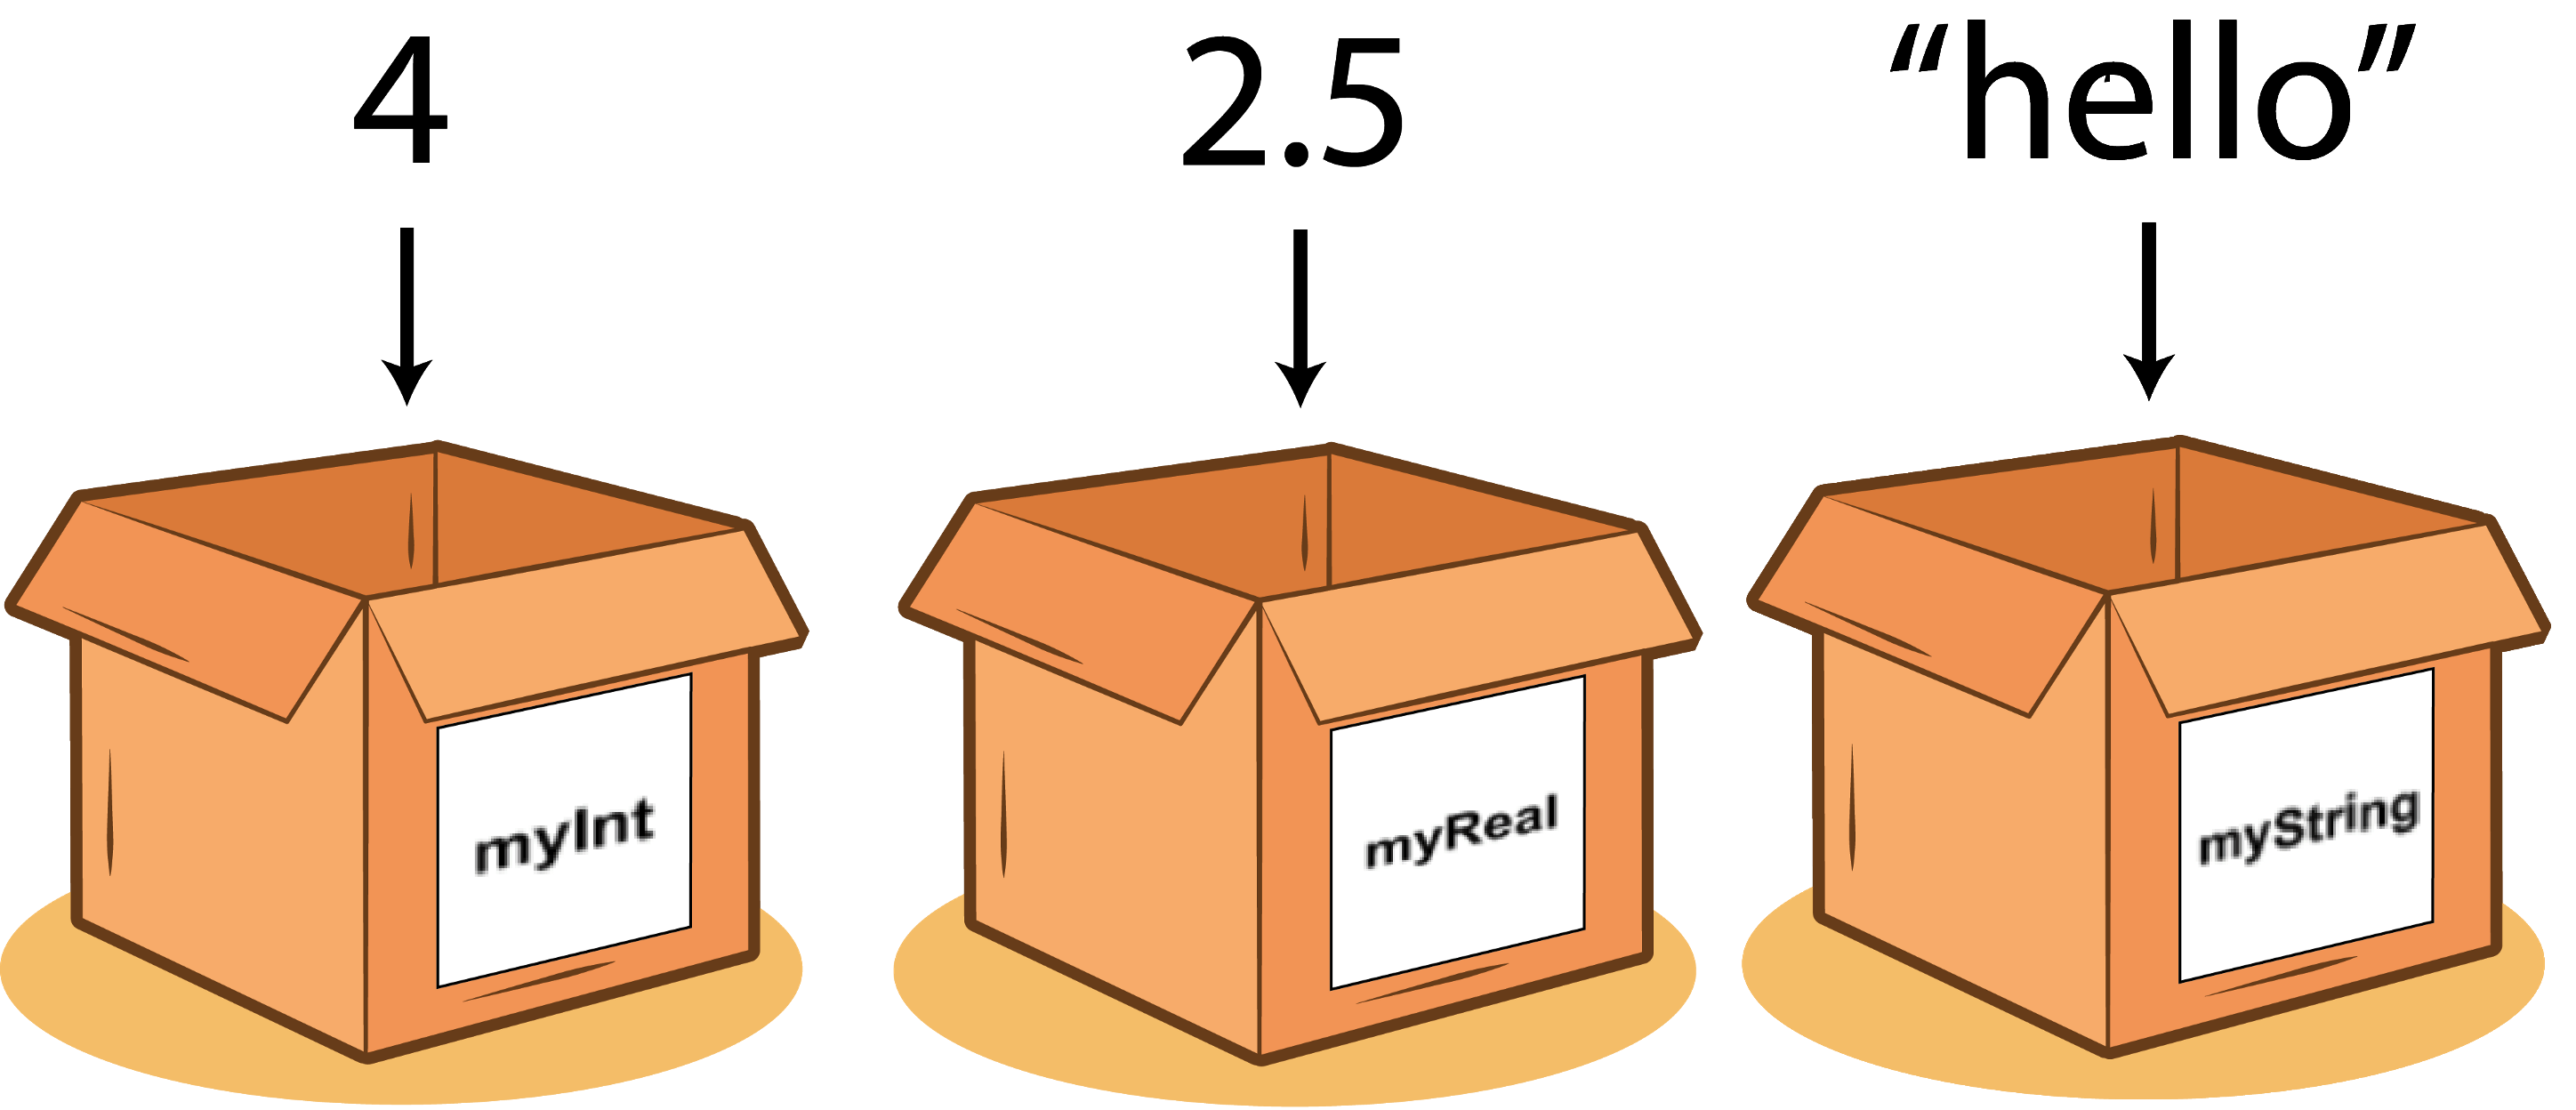
\includegraphics[trim=0 0 0 45,width=0.4\textwidth]{Images/variables/variables2}
\end{center}

\begin{important}
	En \py, les noms de variables doivent en outre obéir à quelques règles simples :\\
	\begin{itemize}
		\item Il est exclusivement composé de lettres (majuscules  et/ou minuscules) et de chiffres mais qui doit toujours	commencer par une lettre.
		\item On ne peut pas utiliser l’un des 33 mots réservés du langage Python
		\begin{multicols}{7}
			\lstinline{and}\\      \lstinline{as}\\         \lstinline{assert}\\      \lstinline{break}\\       \lstinline{class}\\       \lstinline{continue}\\       \lstinline{def}\\
			\lstinline{del}\\       \lstinline{elif}\\       \lstinline{else}\\        \lstinline{except}\\      \lstinline{False}\\       \lstinline{finally}\\        \lstinline{for}\\
			\lstinline{from}\\      \lstinline{global}\\     \lstinline{if}\\          \lstinline{import}\\      \lstinline{in}\\          \lstinline{is}\\             \lstinline{lambda}\\
			\lstinline{None}\\      \lstinline{nonlocal}\\   \lstinline{not}\\         \lstinline{or}\\          \lstinline{pass}\\        \lstinline{raise}\\          \lstinline{return}\\
			\lstinline{True}\\      \lstinline{try}\\        \lstinline{while}\\     \lstinline{with}\\ \lstinline{yield}
		\end{multicols}	
		\item Le Seul symbole autorisé est souligné "$\_$" (underscore en anglais).
		Tous les autres caractères spéciaux sont interdits, en particulier l’espace blanc " " !
		\item Il est sensible à la casse : les minuscules sont différentes des MAJUSCULES. Exemple : les identifiant \lstinline{Age} et \lstinline{age} vont désigner des variables différentes.
	\end{itemize}
\end{important}

\begin{eclairage}
	Il est très important de donner un nom clair et précis aux variables. En lisant le nom de la variable, il faudrait avoir une idée de ce qu'elle représente.
	Par exemple, si je lis \lstinline{note_eleve_JohanS}, je me dis que cette variable représente la note de l'élève Johan S. et donc c'est probablement un \lstinline{float} entre 0.0 et 6.0. Pour améliorer la lecture, on utilise le seul symbole autorisé l'\textit{underscore} "$\_$"\\
\end{eclairage}


\section{L'affectation}
Chaque variable (déclarée) possède une valeur qui est l’information qu’elle porte. Par exemple, la valeur de la variable \lstinline{nombre_eleves_GR103} pourrait être 23, celle de la variable \lstinline{note} pourrait être 4.5, celle de la variable \lstinline{prenom} pourrait être "Anouk".
En \py, pour définir ou modifier la valeur d’une variable, il suffit de lui affecter une valeur en utilisant le symbole égal "\lstinline{=}". 
\begin{mydefinition}
	L’\textbf{affectation} d’une valeur à une variable est l’instruction basique qui permet d’attribuer une valeur à une variable. Par abus de langage, on dit souvent «affectation de variable» ou «assignation de variable».
\end{mydefinition}
En Python, l'affectation s’effectue avec l’opérateur \lstinline{=}. L'instruction d'affectation est composée d'une variable, suivi du symbole égal  \lstinline{=} et d'une expression à évaluer. Après avoir exécutée une affectation la variable prendra la valeur de l'expression évaluée.
\begin{myexample}
	\vspace*{-10px}
	\begin{lstlisting}[numbers=none]
>>> x = (1 + 2) * (3 + 4)
>>> print(x)
21
	\end{lstlisting}\vspace*{-10px}
\end{myexample}

\begin{important}
	\begin{itemize}
		\item 	Il ne faut pas confonde l'opérateur \lstinline{=} (l'affectation) de  l'opérateur \lstinline{==} qui sert à tester l'égalité de deux valeurs. L'opérateur \lstinline{==} est beaucoup plus proche du concept d'égalité utilisée en mathématiques.
		\item l est important de distinguer les expressions, comme \lstinline{x + 2} , des instructions, comme \lstinline{y = x + 2}; . Une expression se calcule, une instruction s’exécute.
	\end{itemize}
	
\end{important}

\subsection{Différents types d’affectations}

\begin{myexamples}
	\itemb{Affectation d'une quantité}
	\begin{lstlisting}[numbers=none]
note = 37 * 50 + 1
	\end{lstlisting}
	\textbf{Explications :}
	\begin{minipage}[t]{0.83\linewidth}
		La valeur \lstinline{37* 50 + 1} (c'est-à-dire \lstinline{4.7}) est injectée dans la case mémoire nommée \lstinline{note}.
	\end{minipage}	
	
	\itemb{Affectation d’un texte}
	\begin{lstlisting}[numbers=none]
prenom = "Robert"
nom_prenom = "Dupont"+'Robert'
	\end{lstlisting}
	\textbf{Remarque :}
	\begin{minipage}[t]{0.85\linewidth}
		Un Chaîne de caractères peut être écrite soit entre "guillemets", soit entre 'apostrophes' droits.
	\end{minipage}
	
	
	\itemb{Affectations parallèles}
	\begin{lstlisting}[numbers=none]
n, x = 1, 7.3
	\end{lstlisting}
	\textbf{Explications :}
	\begin{minipage}[t]{0.83\linewidth}
		C'est équivalent à effectuer les affectations \lstinline{n = 1} et  \lstinline{x = 7.3} simultanément.
	\end{minipage}	
	
	
	\itemb{Auto-affectation}
	\begin{lstlisting}[numbers=none]
k = k ** 2
t = 3 * t - 2
	\end{lstlisting}
	\textbf{Explications :}
	\begin{minipage}[t]{0.83\linewidth}
		Une expression avec la valeur de la variable est calculée puis réaffectée à la variable elle-même.\\
		Par exemple, si \lstinline{t} contient la valeur $5$ alors après avoir exécute \lstinline{t=3*t-2} \lstinline{t} vaudra  \lstinline{3*5-2} (c'est-à-dire \lstinline{13}). 
	\end{minipage}
	
	
	
	\itemb{Incrémentation ou décrémentation}
	\begin{lstlisting}[numbers=none]
k = k + 1
compteur = compteur - 2
	\end{lstlisting}
	\textbf{Remarque :}
	\begin{minipage}[t]{0.85\linewidth}
		Auto-affectation additionnée ou soustraite d’un certain \textit{pas} (d’un certain nombre) entier.
	\end{minipage}
\end{myexamples}